\section{N : Recursion}
\label{chap:recurs}

%%%%%%%%%%%%%%%%%%%%%%%%%%%%%%%%%%%%%%%%%%%%%%%%%%%%%%%%%%%%%%

\begin{frame}[fragile]
\frametitle{Simple Recursion}
\begin{columns}[T]

\begin{column}{0.45\textwidth}
\begin{itemize}[<+->]
\item When a function calls itself, this is known as recursion.
\item This is an important theme in Computer Science that crops up
time \& time again.
\item Can sometimes lead to very simple and elegant programs.
\item Let's look at some toy examples to begin with.
\end{itemize}
\end{column}

\pause
\begin{column}{0.45\textwidth}
\lstinputlisting[style=basicc]{../Code/ChapN/strrev_it.c}
\outputlisting{../Code/ChapN/strrev_it.autoout}
\end{column}

\end{columns}
\end{frame}

%%%%%%%%%%%%%%%%%%%%%%%%%%%%%%%%%%%%%%%%%%%%%%%%%%%%%%%%%%%%%%

\begin{frame}[fragile]
\frametitle{Recursion for {\em strrev()}}

\begin{columns}[T]

\begin{column}{0.45\textwidth}
\lstinputlisting[style=basicc]{../Code/ChapN/strrev_rec.c}
\outputlisting{../Code/ChapN/strrev_rec.autoout}
\end{column}

\pause
\begin{column}{0.45\textwidth}
\begin{itemize}[<+->]
\item We need to change the function prototype.
\item This allows us to track both the start and the end of the string.
\end{itemize}
\end{column}

\end{columns}
\end{frame}

%%%%%%%%%%%%%%%%%%%%%%%%%%%%%%%%%%%%%%%%%%%%%%%%%%%%%%%%%%%%%%

\begin{frame}[fragile]
\frametitle{The Fibonacci Sequence}
\begin{columns}[T]


\begin{column}{0.35\textwidth}
A well known example of a recursive function is the Fibonacci
sequence. The first term is 1, the second term is 1 and each
successive term is defined to be the sum of the two previous
terms, i.e. :
\begin{verbatim}
fib(1) is 1
fib(2) is 1
fib(n) is fib(n-1)+fib(n-2)

1,1,2,3,5,8,13,21, ...
\end{verbatim}
\end{column}

\end{columns}
\end{frame}

%%%%%%%%%%%%%%%%%%%%%%%%%%%%%%%%%%%%%%%%%%%%%%%%%%%%%%%%%%%%%%

\begin{frame}[fragile]
\frametitle{Iterative \& Recursive Fibonacci}
\begin{columns}[T]

\begin{column}{0.50\textwidth}
\lstinputlisting[style=basicc]{../Code/ChapN/fib_it.c}
\end{column}

\pause
\begin{column}{0.40\textwidth}
\outputlisting{../Code/ChapN/fib_it.autoout}
\end{column}

\end{columns}
\end{frame}

%%%%%%%%%%%%%%%%%%%%%%%%%%%%%%%%%%%%%%%%%%%%%%%%%%%%%%%%%%%%%%

\begin{frame}[fragile]
\frametitle{Iterative \& Recursive Fibonacci}
\begin{columns}[T]

\begin{column}{0.50\textwidth}
\lstinputlisting[style=basicc]{../Code/ChapN/fib_rec.c}
\end{column}

\pause
\begin{column}{0.40\textwidth}
It's interesting to see how run-time increases as the length of the sequence is raised.
\begin{figure}[h]
\centerline{
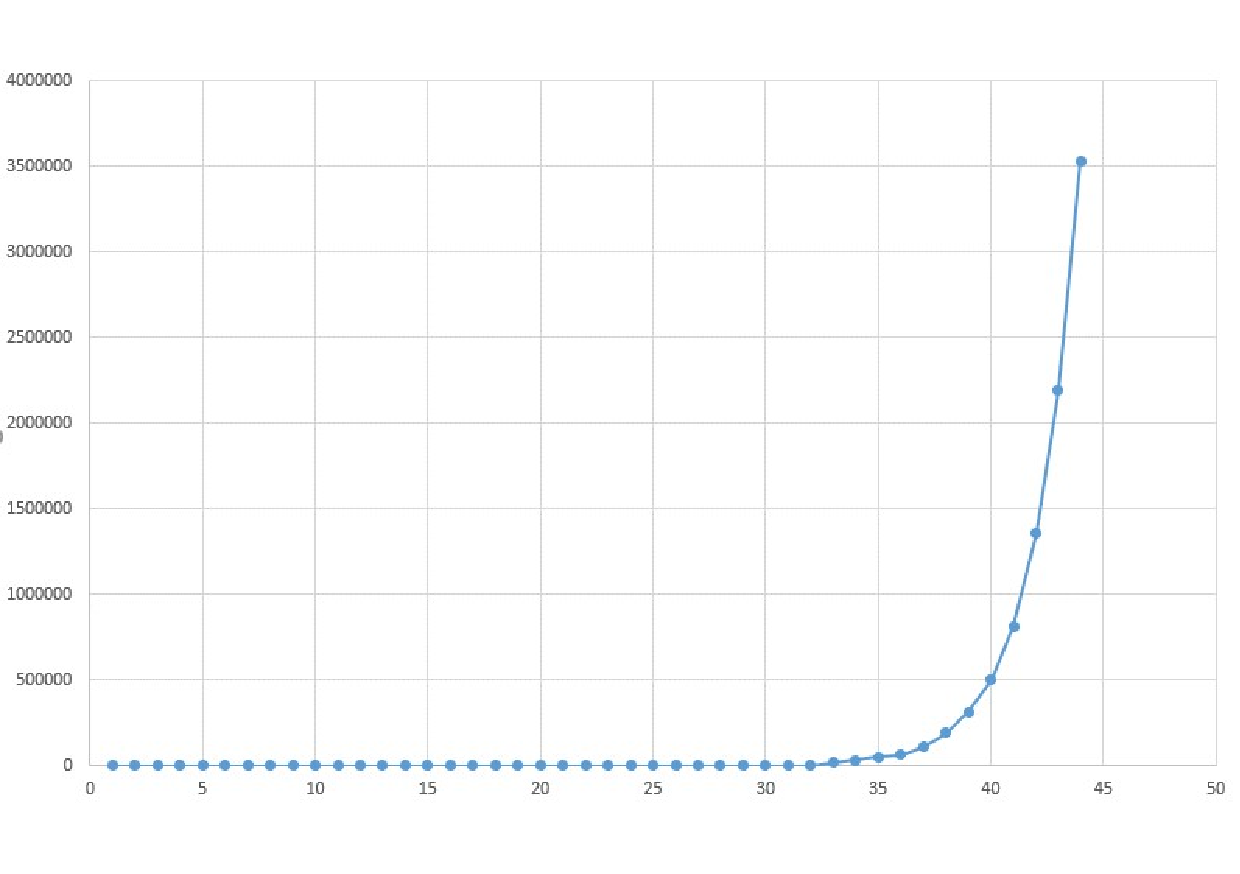
\includegraphics[scale=0.25]{../Images/fib_timer.pdf}
}
\end{figure}
\end{column}

\end{columns}
\end{frame}

%%%%%%%%%%%%%%%%%%%%%%%%%%%%%%%%%%%%%%%%%%%%%%%%%%%%%%%%%%%%%%

\begin{frame}[fragile]
\frametitle{Maze Escape}
\begin{columns}[T]

\begin{column}{0.45\textwidth}
The correct route through a maze can be obtained via
recursive, rather than iterative, methods.
\begin{center}
\begin{tikzpicture}
    [%%%%%%%%%%%%%%%%%%%%%%%%%%%%%%
        box/.style={rectangle,draw=black,thick, minimum size=1cm},
    ]%%%%%%%%%%%%%%%%%%%%%%%%%%%%%%

\foreach \x in {0,1,...,4}{
    \foreach \y in {0,1,...,4}
        \node[box] at (\x,\y){};
}
\node[box,fill=britishrg] at (0,4){};  
\node[box,fill=britishrg] at (2,4){};  
\node[box,fill=britishrg] at (3,4){};  
\node[box,fill=britishrg] at (4,4){};  
\node[box,fill=britishrg] at (0,3){};  
\node[box,fill=britishrg] at (4,3){};  
\node[box,fill=britishrg] at (0,2){};  
\node[box,fill=britishrg] at (1,2){};  
\node[box,fill=britishrg] at (2,2){};  
\node[box,fill=britishrg] at (4,2){};  
\node[box,fill=britishrg] at (0,1){};  
\node[box,fill=britishrg] at (4,1){};  
\node[box,fill=britishrg] at (0,0){};  
\node[box,fill=britishrg] at (2,0){};  
\node[box,fill=britishrg] at (3,0){};  
\node[box,fill=britishrg] at (4,0){};  
\end{tikzpicture}
\end{center}
\end{column}

\pause
\begin{column}{0.45\textwidth}
{\small
\begin{verbatim}
bool explore(int x, int y, char mz[YS][XS])
{
   if  mz[y][x] is exit return true;

   Mark mz[y][x] so we don't return here

   if we can go up :
      if(explore(x, y+1, mz)) return true

   if we can go right :
      if(explore(x+1, y, mz)) return true

   Do left & down in a similar manner

   return false; // Failed to find route
}
\end{verbatim}
}
\end{column}

\end{columns}
\end{frame}

%%%%%%%%%%%%%%%%%%%%%%%%%%%%%%%%%%%%%%%%%%%%%%%%%%%%%%%%%%%%%%

\begin{frame}[fragile]
\frametitle{Permuting}
\begin{columns}[T]

\begin{column}{0.40\textwidth}
\begin{itemize}[<+->]
\item Here we consider the ways to permute a string (or more generally an array)
\item Permutations are all possible ways of rearranging the positions of the characters.

\outputlisting{../Code/ChapN/permute.autoout}
\end{itemize}
\end{column}

\pause
\begin{column}{0.50\textwidth}
\lstinputlisting[style=basicc]{../Code/ChapN/permute.c}
\end{column}

\end{columns}
\end{frame}

%%%%%%%%%%%%%%%%%%%%%%%%%%%%%%%%%%%%%%%%%%%%%%%%%%%%%%%%%%%%%%

\begin{frame}[fragile]
\frametitle{Self-test : Power}
\begin{columns}[T]

\begin{column}{0.45\textwidth}
\begin{itemize}[<+->]
\item Raising a number to a power \verb$n = 2^5$ is the same
as multiple multiplications \verb^n = 2*2*2*2*2^.
\item Or, thinking recursively, \verb$n = 2 * (2^4)$.
\end{itemize}
\end{column}

\pause
\begin{column}{0.45\textwidth}
\lstinputlisting[style=basicc]{../Code/ChapN/power.c}
\end{column}

\end{columns}
\end{frame}
